\documentclass[11pt]{article}

% ---------------------------------------------------------------- packages
\usepackage[margin=1in]{geometry}
\usepackage[T1]{fontenc}
\usepackage{mathptmx}                 % Times
\usepackage{amsmath,amssymb}
\usepackage{booktabs}
\usepackage{microtype}
\usepackage[font=small,labelfont=bf,skip=4pt]{caption}
\usepackage{enumitem}
\setlist{noitemsep,topsep=2pt,leftmargin=*}
\usepackage[numbers,sort&compress,square]{natbib}
\usepackage{xcolor}
\usepackage{titlesec}
\titlespacing*{\section}{0pt}{8pt plus 2pt}{3pt}
\usepackage{pgfplots}
\pgfplotsset{compat=1.16}
\usepackage[colorlinks=true,linkcolor=black,citecolor=blue!60!black,urlcolor=blue!60!black]{hyperref}

\setlength{\parskip}{3pt}
\setlength{\parindent}{0pt}
\setlength{\textfloatsep}{8pt plus 2pt}
\setlength{\intextsep}{6pt plus 2pt}
\setlength{\abovedisplayskip}{4pt}
\setlength{\belowdisplayskip}{4pt}

% ---------------------------------------------------------------- title
\title{\vspace{-2.0cm}\textbf{CS6315E NEURAL NETWORKS AND DEEP LEARNING}\\[4pt]
       \Large RTE Challenge}
\author{Prakash Roy}
\date{}

\begin{document}
\maketitle
\vspace{-1.5cm}

\begin{abstract}
\noindent This report addresses Recognizing Textual Entailment (RTE) under a joint accuracy--size criterion.
ALBERT-large-v2 (17.7M parameters) is fine-tuned with FreeLB adversarial training, which raises dev accuracy from
80.5\% to 82.5\% over five seeds ($p=0.02$) at no parameter cost; the submitted model reaches 82.3\%. Distillation
adds stability but not accuracy, and larger models buy at most 4--8 points at 10--25$\times$ the parameters.
\end{abstract}

% ================================================================ 1
\section{Approach}

\textbf{Task and data.} RTE \cite{dagan2006pascal,wang2019glue} is a binary task: given a premise and a hypothesis, decide
whether the hypothesis follows from the premise (\emph{entailment} or \emph{not entailment}). The 2,490 training pairs are split into 2,241 for training and a
stratified hold-out of 249 (seed 1234). The hold-out selects checkpoints and ranks training recipes; the 277 dev
pairs are only used for reporting.

\textbf{Model and why.} Because model size is weighed alongside accuracy, the model is ALBERT-large-v2
\cite{lan2020albert}. Cross-layer parameter sharing and factorised 128-dimensional embeddings give it the depth of
a 24-layer, 1024-wide transformer (16 heads, feed-forward size 4096, 30k SentencePiece vocabulary) with only 17.7M
parameters, about 6$\times$ fewer than BERT-base \cite{devlin2019bert}. Each pair is encoded as
``[CLS] premise [SEP] hypothesis [SEP]'' (at most 256 tokens), and the pooled [CLS] vector feeds a new linear
layer with two outputs. All weights are fine-tuned: 17,686,018 parameters, all trainable (no adapters or LoRA).

\textbf{Fine-tuning strategy.} Cross-entropy loss, AdamW \cite{loshchilov2019adamw} with learning rate $10^{-5}$
and weight decay 0.01, batch size 16, 10 epochs, linear warm-up over the first 25\% of steps and linear decay,
gradient clipping at 1.0 and fp16 mixed precision. On top of this, FreeLB \cite{zhu2020freelb} trains
on adversarially perturbed word embeddings $E(X)$. The training objective is
\begin{equation}
\min_\theta\; \mathbb{E}_{(X,y)}\Big[\frac{1}{K}\sum_{k=0}^{K-1}\mathcal{L}\big(f_\theta(E(X)+\delta_k),\,y\big)\Big],
\label{eq:obj}
\end{equation}
where each perturbation is found by normalised gradient ascent:
\begin{align}
g_k &= \nabla_{\delta}\,\mathcal{L}\big(f_\theta(E(X)+\delta_k),\,y\big), \label{eq:grad}\\
\delta_{k+1} &= \delta_k + \alpha\,\lVert e\rVert\,\frac{g_k}{\lVert g_k\rVert}. \label{eq:step}
\end{align}
The settings are $K=2$ ascent steps, a random start $\delta_0$ of norm $0.01\lVert e\rVert$ and $\alpha=0.03$, where
$\lVert e\rVert$ is the norm of each token's embedding. The parameter gradients of all $K$ passes in
Eq.~\eqref{eq:obj} are accumulated, so the model learns to keep its answer under small worst-case changes of its input.

\textbf{Training recipes compared.} All keep the same 17.7M-parameter model:
\begin{itemize}
  \item \emph{long}: 20 epochs, the stable fine-tuning recipe of Mosbach et al.~\cite{mosbach2021stability}.
  \item \emph{SMART}: the smoothness-inducing adversarial penalty of Jiang et al.~\cite{jiang2020smart}.
  \item \emph{kd}: knowledge distillation \cite{hinton2015distilling} from an ensemble of three DeBERTa-v3-large
        runs \cite{he2023debertav3} trained on the same split, using the gold pairs plus four teacher-labelled copies of
        each pair with words randomly deleted or masked ($p=0.15$); loss $0.7\,T^2\,\mathrm{KL}+0.3\,\mathrm{CE}$, $T=2$.
  \item \emph{self}: born-again distillation \cite{furlanello2018born}, with an ensemble of three FreeLB
        ALBERT-large runs as the teacher; \emph{kd+FreeLB} and \emph{self+FreeLB} add FreeLB.
\end{itemize}

\textbf{Protocol.} Every recipe is trained with five seeds (42--46). A run keeps the epoch with the best hold-out
accuracy and is evaluated once on dev; it counts as failed if its gold-label training loss at that checkpoint is
still $\ge 0.5$. Results are reported as mean $\pm$ standard deviation over seeds, and dev accuracies are compared with plain fine-tuning
using Welch's $t$-test \cite{welch1947}. Implementation: PyTorch \cite{paszke2019pytorch} and Hugging Face
Transformers \cite{wolf2020transformers} on Kaggle T4 GPUs.

% ================================================================ 2
\section{Results}

\begin{table}[h]
\centering\small
\caption{ALBERT-large-v2 (17.7M parameters) with different training recipes, 5 seeds each (mean $\pm$ sd).}
\label{tab:recipes}
\begin{tabular}{lccc}
\toprule
Recipe & Hold-out acc.\ (\%) & Dev acc.\ (\%) & Dev vs.\ plain ($p$) \\
\midrule
plain fine-tuning (baseline) & 83.8 $\pm$ 1.4 & 80.5 $\pm$ 1.2 & --- \\
long (20 epochs)             & 83.2 $\pm$ 0.3 & 79.4 $\pm$ 0.7 & $-1.2$ (0.10) \\
\textbf{FreeLB}              & \textbf{86.3 $\pm$ 1.3} & \textbf{82.5 $\pm$ 0.9} & \textbf{+1.9 (0.02)} \\
SMART                        & 85.4 $\pm$ 1.9 & 80.6 $\pm$ 2.5 & +0.1 (0.96) \\
kd (1 of 5 runs failed)      & 82.5 $\pm$ 1.8 & 81.2 $\pm$ 0.9 & +0.7 (0.33) \\
kd + FreeLB                  & 83.8 $\pm$ 0.5 & 82.5 $\pm$ 0.7 & +1.9 (0.02) \\
self                         & 83.8 $\pm$ 3.2 & 81.9 $\pm$ 2.7 & +1.4 (0.31) \\
self + FreeLB                & 85.5 $\pm$ 1.3 & 82.2 $\pm$ 0.7 & +1.7 (0.03) \\
\midrule
\textit{Teacher: DeBERTa-v3-large (435.1M)} & \textit{90.8 $\pm$ 1.2} & \textit{90.0 $\pm$ 0.8} & --- \\
\bottomrule
\end{tabular}
\end{table}

\begin{figure}[h]
\centering
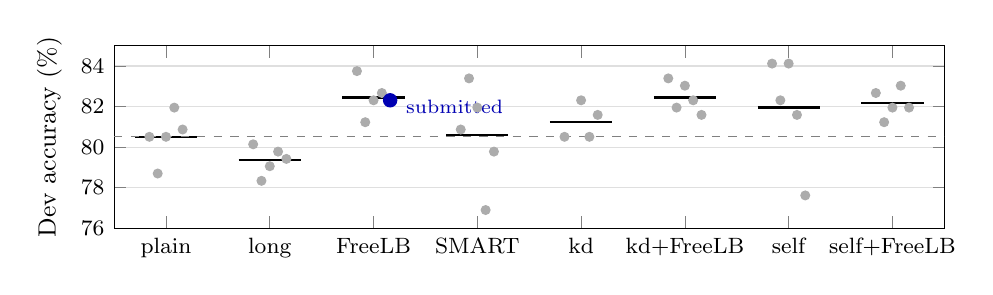
\begin{tikzpicture}
\begin{axis}[
    width=\linewidth, height=3.9cm,
    xmin=0.5, xmax=8.5, ymin=76, ymax=85,
    xtick={1,...,8},
    xticklabels={plain, long, FreeLB, SMART, kd, kd+FreeLB, self, self+FreeLB},
    ytick={76,78,80,82,84}, ylabel={Dev accuracy (\%)},
    ymajorgrids, grid style={gray!25},
    tick label style={font=\footnotesize}, label style={font=\small},
]
\addplot[only marks, mark=*, mark size=1.6pt, gray!65] coordinates {
 (0.84,80.51) (0.92,78.7) (1,80.51) (1.08,81.95) (1.16,80.87)
 (1.84,80.14) (1.92,78.34) (2,79.06) (2.08,79.78) (2.16,79.42)
 (2.84,83.75) (2.92,81.23) (3,82.31) (3.08,82.67)
 (3.84,80.87) (3.92,83.39) (4,81.95) (4.08,76.9) (4.16,79.78)
 (4.84,80.51) (5,82.31) (5.08,80.51) (5.16,81.59)
 (5.84,83.39) (5.92,81.95) (6,83.03) (6.08,82.31) (6.16,81.59)
 (6.84,84.12) (6.92,82.31) (7,84.12) (7.08,81.59) (7.16,77.62)
 (7.84,82.67) (7.92,81.23) (8,81.95) (8.08,83.03) (8.16,81.95)};
\addplot[only marks, mark=*, mark size=2.4pt, blue!70!black] coordinates {(3.16,82.31)};
\foreach \x/\m in {1/80.51, 2/79.35, 3/82.45, 4/80.58, 5/81.23, 6/82.45, 7/81.95, 8/82.17}{
  \edef\temp{\noexpand\draw[black, thick] (axis cs:\x-0.3,\m) -- (axis cs:\x+0.3,\m);}\temp }
\draw[dashed, gray] (axis cs:0.5,80.51) -- (axis cs:8.5,80.51);
\node[font=\scriptsize, blue!70!black, anchor=west] at (axis cs:3.22,82.0) {submitted};
\end{axis}
\end{tikzpicture}
\caption{Dev accuracy of every run (dots, 5 seeds per recipe) with the recipe mean (bar); dashed line: plain
fine-tuning mean. The failed kd run (61.7\%) is not shown. Blue: the submitted run.}
\label{fig:seeds}
\end{figure}

FreeLB is the only ingredient that reliably helps (Table~\ref{tab:recipes}, Figure~\ref{fig:seeds}): it adds 1.9 dev
points ($p=0.02$) with a narrow spread, and even its worst run (81.2\%) beats the plain fine-tuning mean.
Distillation alone gives +0.7 points (not significant), because the teacher had seen the training pairs and its soft
labels are almost the gold labels; combined with FreeLB it gives the most consistent runs but no extra accuracy.
SMART (seeds from 76.9\% to 83.4\%) and longer training do not help, and averaging the weights of several seeds
(``model soups'' \cite{wortsman2022soups}) gave no gain. The submitted model is the run with the highest hold-out accuracy among all
40 ALBERT-large runs (FreeLB, seed 46); Table~\ref{tab:final} compares it with the baseline.

\begin{table}[h]
\centering\small
\caption{Submitted model vs.\ baseline. Both have the same architecture and size.}
\label{tab:final}
\begin{tabular}{lccc}
\toprule
Model & Parameters (all trainable) & Hold-out acc.\ (\%) & Dev acc.\ (\%) \\
\midrule
\textbf{Submitted: ALBERT-large-v2 + FreeLB} & \textbf{17,686,018} & \textbf{87.6} & \textbf{82.3} \\
FreeLB recipe, mean of 5 seeds          & 17,686,018 & 86.3 $\pm$ 1.3 & 82.5 $\pm$ 0.9 \\
Baseline: plain fine-tuning, mean of 5 seeds & 17,686,018 & 83.8 $\pm$ 1.4 & 80.5 $\pm$ 1.2 \\
\bottomrule
\end{tabular}
\end{table}

% ================================================================ 3
\section{Accuracy vs.\ Parameters}

\begin{figure}[h]
\centering
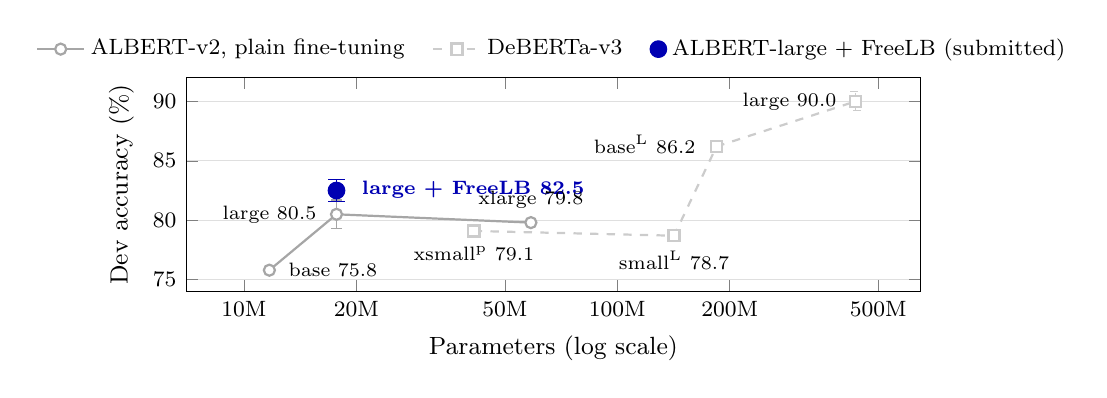
\begin{tikzpicture}
\begin{semilogxaxis}[
    width=0.9\linewidth, height=4.3cm,
    xmin=7, xmax=650, ymin=74, ymax=92,
    xtick={10,20,50,100,200,500}, xticklabels={10M,20M,50M,100M,200M,500M},
    log ticks with fixed point,
    xlabel={Parameters (log scale)}, ylabel={Dev accuracy (\%)},
    ymajorgrids, grid style={gray!25},
    tick label style={font=\footnotesize}, label style={font=\small},
    legend style={font=\footnotesize, at={(0.5,1.03)}, anchor=south, draw=none, fill=none,
                  legend columns=3, /tikz/every even column/.append style={column sep=8pt}},
]
\addplot[gray!70, thick, mark=*, mark options={fill=white}, error bars/.cd, y dir=both, y explicit]
  coordinates {(11.7,75.8) (17.7,80.5) +- (0,1.2) (58.7,79.8)};
\addlegendentry{ALBERT-v2, plain fine-tuning}
\addplot[gray!40, thick, dashed, mark=square*, mark options={fill=white, solid}, error bars/.cd, y dir=both, y explicit]
  coordinates {(41.3,79.1) (141.9,78.7) (184.4,86.2) +- (0,0.5) (435.1,90.0) +- (0,0.8)};
\addlegendentry{DeBERTa-v3}
\addplot[only marks, mark=*, mark size=3pt, blue!70!black, error bars/.cd, y dir=both, y explicit]
  coordinates {(17.7,82.5) +- (0,0.9)};
\addlegendentry{ALBERT-large + FreeLB (submitted)}
\node[font=\scriptsize, anchor=west]  at (axis cs:12.4,75.8) {base 75.8};
\node[font=\scriptsize, anchor=east]  at (axis cs:16.6,80.5) {large 80.5};
\node[font=\scriptsize, anchor=west, blue!70!black] at (axis cs:19.5,82.6) {\textbf{large + FreeLB 82.5}};
\node[font=\scriptsize, anchor=south] at (axis cs:58.7,80.2) {xlarge 79.8};
\node[font=\scriptsize, anchor=north] at (axis cs:41.3,78.6) {xsmall\textsuperscript{p} 79.1};
\node[font=\scriptsize, anchor=north] at (axis cs:141.9,78.2) {small\textsuperscript{L} 78.7};
\node[font=\scriptsize, anchor=east]  at (axis cs:172,86.4) {base\textsuperscript{L} 86.2};
\node[font=\scriptsize, anchor=east]  at (axis cs:410,90.0) {large 90.0};
\end{semilogxaxis}
\end{tikzpicture}
\caption{Dev accuracy vs.\ parameter count for every model trained in this work (labels: model size and dev accuracy). ALBERT-large (plain and FreeLB) and
DeBERTa-large: 5 seeds, mean $\pm$ sd. Other points: earlier runs with 1--5 seeds and plain fine-tuning or LoRA
\cite{hu2022lora} (\textsuperscript{L}); \textsuperscript{p}: after vocabulary pruning.}
\label{fig:size}
\end{figure}

Figure~\ref{fig:size} shows how accuracy scales with size. A \emph{smaller} model would have done worse: ALBERT-base
saves 6.0M parameters but loses 4.7 points. A \emph{larger} ALBERT would not have done better: ALBERT-xlarge has
3.3$\times$ the parameters and scored 0.7 points lower. Only a different model family buys accuracy, at a steep
price in size: DeBERTa-v3-base gains 3.7 points over the submitted model with 10.4$\times$ the parameters, and DeBERTa-v3-large
gains 7.5 points with 24.6$\times$. Two attempts to make models cheaper failed outright (ALBERT with 10\% dropout
added, and DeBERTa-v3-base cut to 6--8 layers, both collapsed to 50--53\%). Since parameter count is part of the
criterion, ALBERT-large is the best trade-off, and the effort went into training it better rather than making it larger.

% ================================================================ 4
\section{Error Analysis}

The submitted model gets 49 of the 277 dev pairs wrong (Figure~\ref{fig:cm}); Table~\ref{tab:errors} breaks its
accuracy down by simple properties of the pairs.

\begin{figure}[h]
\centering
\begin{minipage}[c]{0.6\linewidth}
\centering\small
\captionof{table}{Dev accuracy of the submitted model on slices (one standard error $\approx$ 3 points).}
\label{tab:errors}
\begin{tabular}{lcc}
\toprule
Slice & Pairs & Acc.\ (\%) \\
\midrule
Premise $\le$ 30 words / $>$ 30 words & 135 / 142 & 85.2 / 79.6 \\
Word overlap $\ge$ 80\% / $<$ 80\%   & 87 / 190  & 81.6 / 82.6 \\
Negation word / none                 & 37 / 240  & 81.1 / 82.5 \\
Gold entailment / not\_entailment    & 146 / 131 & 84.9 / 79.4 \\
\bottomrule
\end{tabular}
\end{minipage}\hfill
\begin{minipage}[c]{0.37\linewidth}
\centering
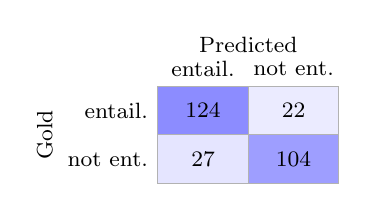
\begin{tikzpicture}[x=1.15cm, y=0.62cm, font=\footnotesize]
\fill[blue!45] (0,1) rectangle (1,2); \node at (0.5,1.5) {124};
\fill[blue!8]  (1,1) rectangle (2,2); \node at (1.5,1.5) {22};
\fill[blue!10] (0,0) rectangle (1,1); \node at (0.5,0.5) {27};
\fill[blue!38] (1,0) rectangle (2,1); \node at (1.5,0.5) {104};
\draw[gray!60] (0,0) rectangle (2,2) (1,0) -- (1,2) (0,1) -- (2,1);
\node[anchor=east] at (0,1.5) {entail.};
\node[anchor=east] at (0,0.5) {not ent.};
\node at (0.5,2.35) {entail.};
\node at (1.5,2.35) {not ent.};
\node at (1,2.85) {Predicted};
\node[rotate=90] at (-1.25,1) {Gold};
\end{tikzpicture}
\captionof{figure}{Confusion matrix (dev).}
\label{fig:cm}
\end{minipage}
\end{figure}

\begin{itemize}
  \item \textbf{Long premises are the clearest weakness} (79.6\% vs.\ 85.2\%): the relevant fact is buried in a longer text.
  \item \textbf{High word overlap does not make a pair easier.} When at least 80\% of the hypothesis words appear in
        the premise, accuracy is slightly lower; these are likely pairs that reuse the premise's words but change
        who did what, a number or a date.
  \item \textbf{Negation is not a weakness} (81.1\% vs.\ 82.5\%), although only 37 dev pairs contain a negation word.
  \item \textbf{The model leans towards entailment}: 27 of its 49 errors are not-entailed pairs that it labelled as
        entailment, i.e.\ it is misled when a hypothesis merely sounds supported by the premise.
\end{itemize}

% ================================================================ 5
\section{Reflection}

With more time and compute, three directions are promising: (i)~an \emph{out-of-fold teacher}, so that every training pair is labelled
by a model that never saw it and its soft labels carry real information; (ii)~\emph{continued pretraining} of ALBERT-large on unlabeled news and
Wikipedia text with replaced-token detection \cite{clark2020electra}, the objective behind DeBERTa-v3
\cite{he2023debertav3}; (iii)~FreeLB on ALBERT-base and ALBERT-xlarge, which were only trained plainly, to re-check the size decision.

% ================================================================ references (numbered in order of first citation)
\begin{thebibliography}{99}
\small

\bibitem{dagan2006pascal}
Ido Dagan, Oren Glickman, and Bernardo Magnini.
\newblock The {PASCAL} recognising textual entailment challenge.
\newblock In \emph{Machine Learning Challenges: Evaluating Predictive Uncertainty, Visual Object Classification,
  and Recognising Textual Entailment}, LNCS 3944, pages 177--190. Springer, 2006.

\bibitem{wang2019glue}
Alex Wang, Amanpreet Singh, Julian Michael, Felix Hill, Omer Levy, and Samuel~R. Bowman.
\newblock {GLUE}: A multi-task benchmark and analysis platform for natural language understanding.
\newblock In \emph{International Conference on Learning Representations (ICLR)}, 2019.

\bibitem{lan2020albert}
Zhenzhong Lan, Mingda Chen, Sebastian Goodman, Kevin Gimpel, Piyush Sharma, and Radu Soricut.
\newblock {ALBERT}: A lite {BERT} for self-supervised learning of language representations.
\newblock In \emph{International Conference on Learning Representations (ICLR)}, 2020.

\bibitem{devlin2019bert}
Jacob Devlin, Ming-Wei Chang, Kenton Lee, and Kristina Toutanova.
\newblock {BERT}: Pre-training of deep bidirectional transformers for language understanding.
\newblock In \emph{Proceedings of NAACL-HLT}, pages 4171--4186, 2019.

\bibitem{loshchilov2019adamw}
Ilya Loshchilov and Frank Hutter.
\newblock Decoupled weight decay regularization.
\newblock In \emph{International Conference on Learning Representations (ICLR)}, 2019.

\bibitem{zhu2020freelb}
Chen Zhu, Yu~Cheng, Zhe Gan, Siqi Sun, Tom Goldstein, and Jingjing Liu.
\newblock {FreeLB}: Enhanced adversarial training for natural language understanding.
\newblock In \emph{International Conference on Learning Representations (ICLR)}, 2020.

\bibitem{mosbach2021stability}
Marius Mosbach, Maksym Andriushchenko, and Dietrich Klakow.
\newblock On the stability of fine-tuning {BERT}: Misconceptions, explanations, and strong baselines.
\newblock In \emph{International Conference on Learning Representations (ICLR)}, 2021.

\bibitem{jiang2020smart}
Haoming Jiang, Pengcheng He, Weizhu Chen, Xiaodong Liu, Jianfeng Gao, and Tuo Zhao.
\newblock {SMART}: Robust and efficient fine-tuning for pre-trained natural language models through principled
  regularized optimization.
\newblock In \emph{Proceedings of ACL}, pages 2177--2190, 2020.

\bibitem{hinton2015distilling}
Geoffrey Hinton, Oriol Vinyals, and Jeff Dean.
\newblock Distilling the knowledge in a neural network.
\newblock \emph{arXiv preprint arXiv:1503.02531}, 2015.

\bibitem{he2023debertav3}
Pengcheng He, Jianfeng Gao, and Weizhu Chen.
\newblock {DeBERTaV3}: Improving {DeBERTa} using {ELECTRA}-style pre-training with gradient-disentangled
  embedding sharing.
\newblock In \emph{International Conference on Learning Representations (ICLR)}, 2023.

\bibitem{furlanello2018born}
Tommaso Furlanello, Zachary~C. Lipton, Michael Tschannen, Laurent Itti, and Anima Anandkumar.
\newblock Born again neural networks.
\newblock In \emph{International Conference on Machine Learning (ICML)}, 2018.

\bibitem{welch1947}
Bernard~L. Welch.
\newblock The generalization of ``{S}tudent's'' problem when several different population variances are involved.
\newblock \emph{Biometrika}, 34(1--2):28--35, 1947.

\bibitem{paszke2019pytorch}
Adam Paszke, Sam Gross, Francisco Massa, Adam Lerer, James Bradbury, Gregory Chanan, et~al.
\newblock {PyTorch}: An imperative style, high-performance deep learning library.
\newblock In \emph{Advances in Neural Information Processing Systems (NeurIPS)}, 2019.

\bibitem{wolf2020transformers}
Thomas Wolf, Lysandre Debut, Victor Sanh, Julien Chaumond, Clement Delangue, Anthony Moi, et~al.
\newblock Transformers: State-of-the-art natural language processing.
\newblock In \emph{Proceedings of EMNLP: System Demonstrations}, pages 38--45, 2020.

\bibitem{wortsman2022soups}
Mitchell Wortsman, Gabriel Ilharco, Samir~Ya Gadre, Rebecca Roelofs, Raphael Gontijo-Lopes, Ari~S. Morcos,
  Hongseok Namkoong, Ali Farhadi, Yair Carmon, Simon Kornblith, and Ludwig Schmidt.
\newblock Model soups: Averaging weights of multiple fine-tuned models improves accuracy without increasing
  inference time.
\newblock In \emph{International Conference on Machine Learning (ICML)}, 2022.

\bibitem{hu2022lora}
Edward~J. Hu, Yelong Shen, Phillip Wallis, Zeyuan Allen-Zhu, Yuanzhi Li, Shean Wang, Lu~Wang, and Weizhu Chen.
\newblock {LoRA}: Low-rank adaptation of large language models.
\newblock In \emph{International Conference on Learning Representations (ICLR)}, 2022.

\bibitem{clark2020electra}
Kevin Clark, Minh-Thang Luong, Quoc~V. Le, and Christopher~D. Manning.
\newblock {ELECTRA}: Pre-training text encoders as discriminators rather than generators.
\newblock In \emph{International Conference on Learning Representations (ICLR)}, 2020.

\end{thebibliography}

\end{document}
